\section{Simple function task}
\subsection{Dataset generation}
\label{sec:appendix:simple-function-task:data-generation}

\begin{figure}[H]
\centering
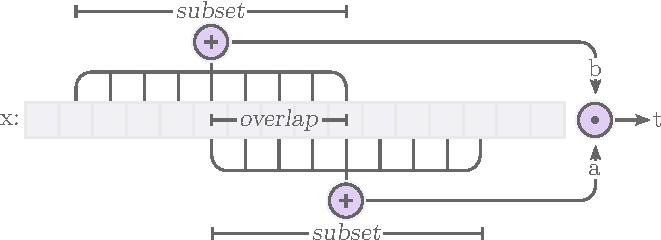
\includegraphics[scale=0.8]{graphics/function_task_static_problem.pdf}
\caption{Dataset is parameterized into ``Input Size'', ``Subset Ratio'', ``Overlap Ratio'', an Operation (here showing multiplication), ``Interpolation Range'' and ``Extrapolation Range'' from which the data set sampled.}
\label{fig:simple-function-task-problem}
\end{figure}

All datasets in the simple function task experiments are generated using the following algorithm:

\begin{algorithm}[H]
  \caption{Dataset sampling algorithm}
  \begin{algorithmic}[1]
    \Function{Dataset}{${\Call{Op}{\cdot, \cdot}: \mathrm{Operation}}$, ${i: \mathrm{Input Size}}$, ${s: \mathrm{Subset Ratio}}$, ${o: \mathrm{Overlap Ratio}}$, ${\hspace{3cm}R: \mathrm{Range}}$}
      \Let{$\mathbf{x}$}{\Call{Uniform}{$R_{lower}, R_{upper}, i$}} \Comment{Sample $i$ elements uniformly}
      \Let{$k$}{\Call{Uniform}{$0, 1 - 2s - o$}} \Comment{Sample offset}
      \Let{$a$}{\Call{Sum}{$\mathbf{x}[ik:i(k+s)]$}} \Comment{Create sum $a$ from subset}
      \Let{$b$}{\Call{Sum}{$\mathbf{x}[i(k+s-o):i (k+2s-0)]$}} \Comment{Create sum $b$ from subset}
      \Let{$t$}{\Call{Op}{$a, b$}} \Comment{Perform operation on $a$ and $b$}
      \State \Return{$x, t$}
    \EndFunction
  \end{algorithmic}
\end{algorithm}

\subsection{Ablation study}
\begin{table}[H]

\caption{\label{tab:function-task-static-ablation}Shows the success-rate for $\mathcal{L}_{\mathbf{W}_1, \mathbf{W}_2} < \mathcal{L}_{\mathbf{W}_1^\epsilon, \mathbf{W}_2^*}$, at what global step the model converged at, and the sparsity error for all weight matrices.}
\centering
\begin{tabular}{rllll}
\toprule
\multicolumn{1}{c}{Model} & \multicolumn{1}{c}{Success} & \multicolumn{2}{c}{Solved at} & \multicolumn{1}{c}{Sparsity error} \\
\cmidrule(l{3pt}r{3pt}){1-1} \cmidrule(l{3pt}r{3pt}){2-2} \cmidrule(l{3pt}r{3pt}){3-4} \cmidrule(l{3pt}r{3pt}){5-5}
 & Rate & Median & Mean & Mean\\
\midrule
$\mathrm{NAC}_{\bullet}$ & $40\%$ & $2.8 \cdot 10^{6}$ & $3.1 \cdot 10^{6} \pm 2.0 \cdot 10^{6}$ & $2.8 \cdot 10^{-2} \pm 8.9 \cdot 10^{-2}$\\

$\mathrm{NAC}_{\bullet}$, $\mathbf{W} = \sigma(\mathbf{\hat{W}})$ & $100\%$ & $1.9 \cdot 10^{6}$ & $1.9 \cdot 10^{6} \pm 3.1 \cdot 10^{5}$ & $1.1 \cdot 10^{-4} \pm 1.0 \cdot 10^{-4}$\\

NMU & $100\%$ & $1.2 \cdot 10^{6}$ & $1.2 \cdot 10^{6} \pm 2.0 \cdot 10^{5}$ & $1.6 \cdot 10^{-3} \pm 9.2 \cdot 10^{-4}$\\

NMU, $\mathbf{W} = \mathbf{\hat{W}}$ & $100\%$ & $1.3 \cdot 10^{6}$ & $1.2 \cdot 10^{6} \pm 1.9 \cdot 10^{5}$ & $3.9 \cdot 10^{-3} \pm 1.2 \cdot 10^{-3}$\\

NMU, $\mathbf{z} = \mathbf{W} \odot \mathbf{x}$ & $100\%$ & $1.2 \cdot 10^{6}$ & $1.2 \cdot 10^{6} \pm 2.0 \cdot 10^{5}$ & $1.6 \cdot 10^{-3} \pm 9.2 \cdot 10^{-4}$\\

NMU, no $\mathcal{R}_{oob}$ & $100\%$ & $1.2 \cdot 10^{6}$ & $1.2 \cdot 10^{6} \pm 1.9 \cdot 10^{5}$ & $1.7 \cdot 10^{-3} \pm 4.6 \cdot 10^{-4}$\\

NMU, no $\mathcal{R}_{sparse},\mathcal{R}_{oob}$ & $100\%$ & $1.1 \cdot 10^{6}$ & $1.1 \cdot 10^{6} \pm 1.8 \cdot 10^{5}$ & $3.3 \cdot 10^{-4} \pm 4.5 \cdot 10^{-5}$\\

NMU, no $\mathcal{R}_{sparse}$ & $100\%$ & $1.2 \cdot 10^{6}$ & $1.2 \cdot 10^{6} \pm 1.9 \cdot 10^{5}$ & $1.7 \cdot 10^{-3} \pm 9.0 \cdot 10^{-4}$\\
\bottomrule
\end{tabular}
\end{table}


\todo[inline]{Remove both regualizers}

\subsubsection{Moments and initialization for addition} \label{sssec:nac-add-moments}

Initialization is important for fast and consistent convergence. The desired properties are according to Glorot et al. \cite{glorot-initialization}:
\begin{equation}
\begin{aligned}
E[z_{h_\ell}] &= 0 & E\left[\frac{\partial \mathcal{L}}{\partial z_{h_{\ell-1}}}\right] &= 0 \\
Var[z_{h_\ell}] &= Var\left[z_{h_{\ell-1}}\right] &
Var\left[\frac{\partial \mathcal{L}}{\partial z_{h_{\ell-1}}}\right] &= Var\left[\frac{\partial \mathcal{L}}{\partial z_{h_{\ell}}}\right]
\end{aligned}
\end{equation}

The $\mathrm{NAU}$ layer is trivial, as this is just a linear layer. Thus the result from Glorot et al. ($Var[W_{h_{\ell-1},h_{\ell}}] = \frac{2}{H_{\ell-1} + H_{\ell}}$) can be used \cite{glorot-initialization}.

However, the original $\mathrm{NAC}_{+}$ unit is less trivial as $W_{h_{\ell-1},h_{\ell}}$ is not sampled directly. Assuming that $\hat{W}_{h_\ell, h_{\ell-1}} \sim \mathrm{Uniform}[-r, r]$ and $\hat{M}_{h_\ell, h_{\ell-1}} \sim \mathrm{Uniform}[-r, r]$ then the variance can be derived (see proof in Appendix \ref{sec:appendix:moments:weight-matrix-construction}) to be:
\begin{equation}
Var[W_{h_{\ell-1},h_{\ell}}] = \frac{1}{2r} \left(1 - \frac{\tanh(r)}{r}\right) \left(r - \tanh\left(\frac{r}{2}\right)\right)
\end{equation}
One can the solve for $r$, given the desired variance.

\subsubsection{Moments and initialization for multiplication} \label{sssec:nac-mul-moments}
\todo{Maybe put this entire section in appendix?}

Using second order multivariate Taylor approximation and some assumptions\todo{put in assumptions in appendix} of uncorrelated stochastic variables, the expectation and variance of the $\mathrm{NAC}_{\bullet}$ layer can be estimated to:
\begin{equation}
\begin{aligned}
f(c_1, c_2) &= \left(1 + c_1 \frac{1}{2} Var[W_{h_\ell, h_{\ell-1}}] \log(|E[z_{h_{\ell-1}}]| + \epsilon)^2\right)^{c_2\ H_{\ell-1}} \\
E[z_{h_\ell}] &\approx f\left(1, 1\right) \\
Var[z_{h_2}] &\approx f\left(4, 1\right) - f\left(1, 2\right) \\
E\left[\frac{\partial \mathcal{L}}{\partial z_{h_{\ell-1}}}\right] &= 0 \\
Var\left[\frac{\partial \mathcal{L}}{\partial z_{h_{\ell-1}}}\right] &\approx Var\left[\frac{\partial \mathcal{L}}{\partial z_{h_{\ell}}}\right] H_{\ell}\ f\left(4, 1\right)\ Var[W_{h_{\ell}, h_{\ell-1}}] \\
&\cdot \left(\frac{1}{\left(|E[z_{h_{\ell-1}}]| + \epsilon\right)^2} + \frac{3}{\left(|E[z_{h_{\ell-1}}]| + \epsilon\right)^4} Var[z_{h_{\ell-1}}]\right)
\end{aligned}
\end{equation}

This is problematic because $E[z_{h_\ell}] \ge 1$, and the variance explodes for $E[z_{h_{\ell-1}}] = 0$ which is normally a desired property.

For our proposed NMU, the expectation and variance can be derived (see proof in Appendix \ref{sec:appendix:moments:nmu}) using the same assumptions as before, although no Taylor approximation is required:
\begin{equation}
\begin{aligned}
E[z_{h_\ell}] &\approx \left(\frac{1}{2}\right)^{H_{\ell-1}} \\
E\left[\frac{\partial \mathcal{L}}{\partial z_{h_{\ell-1}}}\right] &\approx 0 \\
Var[z_{h_\ell}] &\approx \left(Var[W_{h_{\ell-1},h_\ell}] + \frac{1}{4}\right)^{H_{\ell-1}} \left(Var[z_{h_{\ell-1}}] + 1\right)^{H_{\ell-1}} - \left(\frac{1}{4}\right)^{H_{\ell-1}} \\
Var\left[\frac{\partial \mathcal{L}}{\partial z_{h_{\ell-1}}}\right] &\approx Var\left[\frac{\partial \mathcal{L}}{\partial z_{h_\ell}}\right] H_\ell \\
& \cdot \left( \left(Var[W_{h_{\ell-1},h_\ell}] + \frac{1}{4}\right)^{H_{\ell-1}} \left(Var[z_{h_{\ell-1}}] + 1\right)^{H_{\ell-1}-1} - \left(\frac{1}{4}\right)^{H_{\ell-1}}\right)
\end{aligned}
\end{equation}\todo{consider throwing in appendix}

These expectations are much more well behaved. It is properly unlikely to expect that the expectation can become zero, since the identity for multiplication is 1. However, for a large $H_{\ell-1}$ it will be near zero.

The variance is also more well-behaved, but does not provide a input-independent initialization strategy. We propose initializing with $Var[W_{h_{\ell-1},h_\ell}] = \frac{1}{4}$, as this is the solution to $Var[z_{h_\ell}] = Var[z_{h_{\ell-1}}]$ assuming $Var[z_{h_{\ell-1}}] = 1$ and a large $H_{\ell-1}$ (see proof in Appendix \ref{sec:appendix:moments:nmu:initialization}). However, feel free to compute more exact solutions.